% Chapter 4: Static Morphology Across Scientific Fields

\section{Exploratory Metric Diagnostics}

Before comparing fields, I inspect the raw distributions of the eight structural metrics. Their shapes differ clearly. Centroid-distance IQR is right-skewed, kNN distance CV has a visible upper tail, and PCA D80 is partly discrete. The remaining metrics are more symmetric, although they also contain a small number of extreme values. These differences support the use of median/IQR scaling. This makes metrics with different ranges comparable and prevents a few extreme subfields from determining the scale, while keeping those unusual cases visible in the analysis.

\begin{figure}[H]
\centering
\caption[Raw structural metric distributions]{Raw subfield distributions of the eight structural morphology metrics. Dashed vertical lines mark medians.}
\label{fig:structural_metric_raw_distributions}
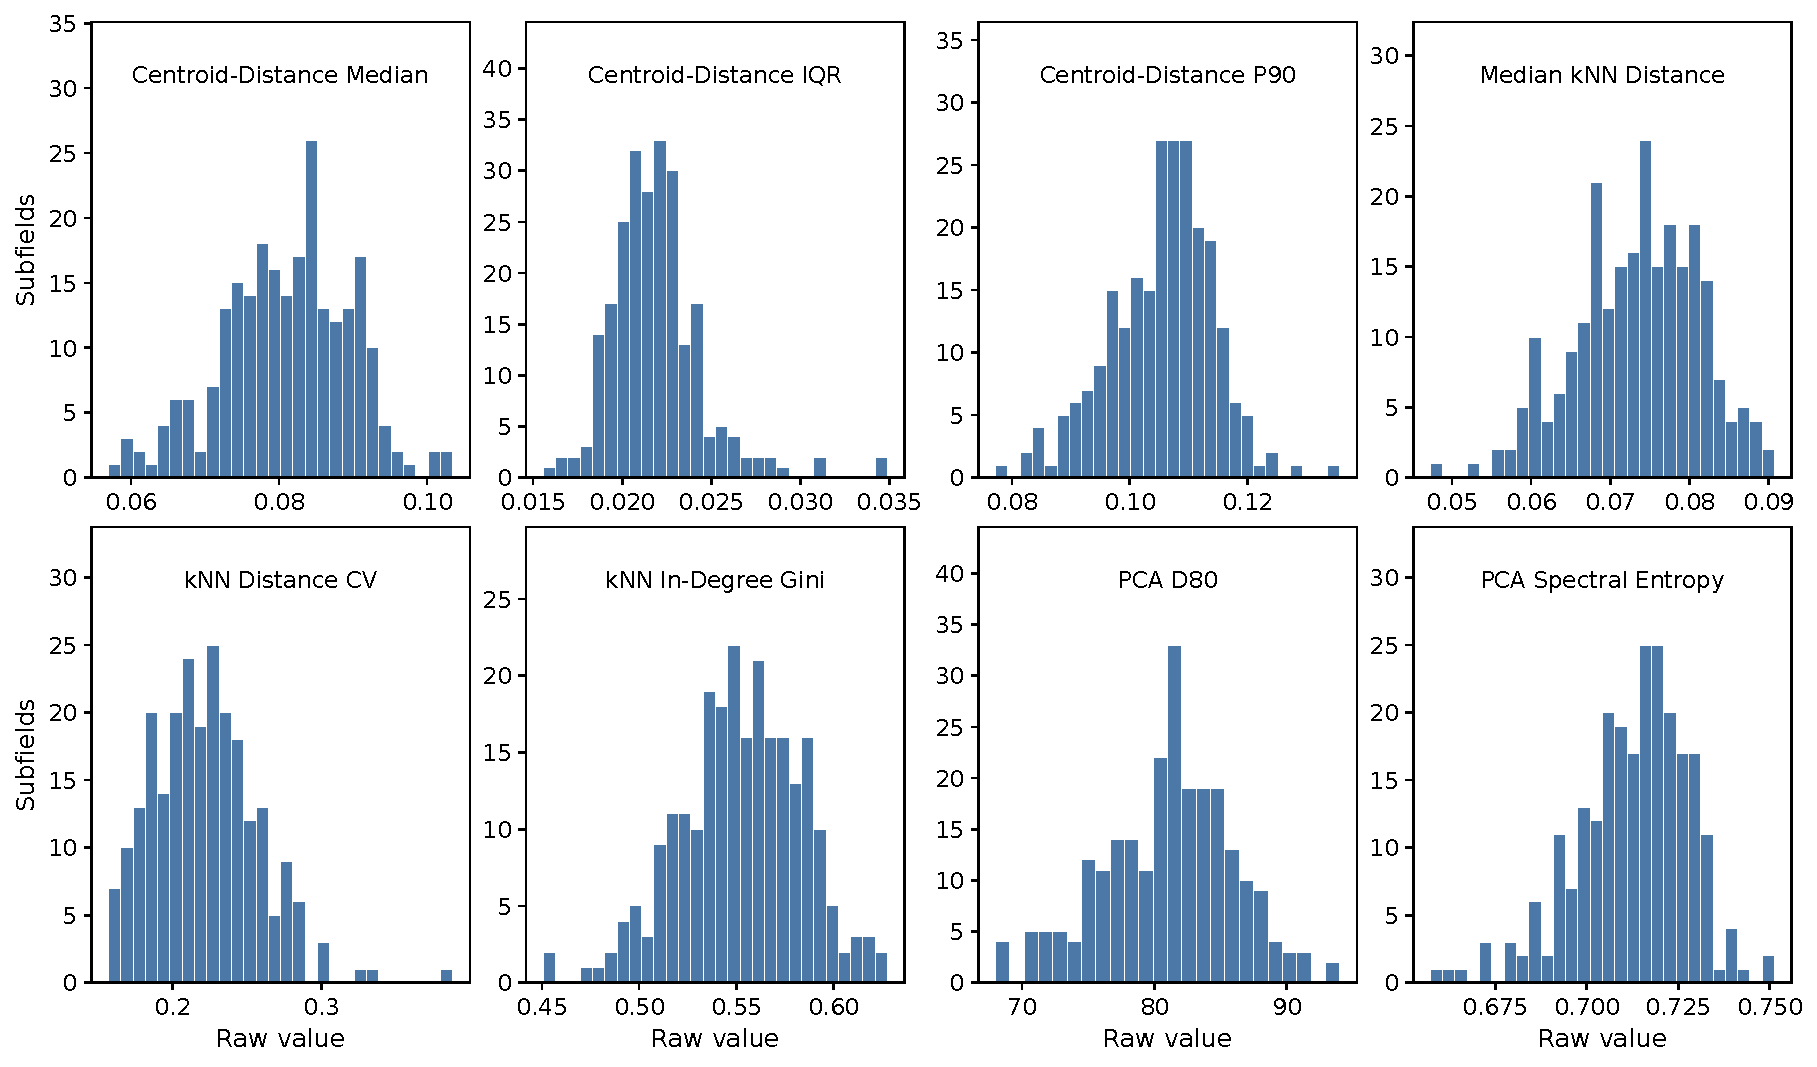
\includegraphics[width=\textwidth]{figures/fig_06_structural_metric_raw_distributions.pdf}
\end{figure}

The correlations show that some metrics are related, but the families are not redundant. Centroid median and centroid P90 are strongly correlated (\(\rho=0.883\)), as expected for two measures of radial spread. PCA \(D_{80}\) and PCA entropy are also strongly related (\(\rho=0.856\)), because both summarize the variance spectrum. The largest negative relation is between kNN median distance and kNN CV (\(\rho=-0.798\)): subfields with closer local neighborhoods often have more uneven local packing. Correlations across different families are weaker. This supports keeping global dispersion, local density, hubness, and spectral structure as separate dimensions.

\begin{figure}[H]
\centering
\caption[Structural metric Spearman correlations]{Spearman correlation matrix for the eight raw structural morphology metrics.}
\label{fig:structural_metric_spearman_correlation}
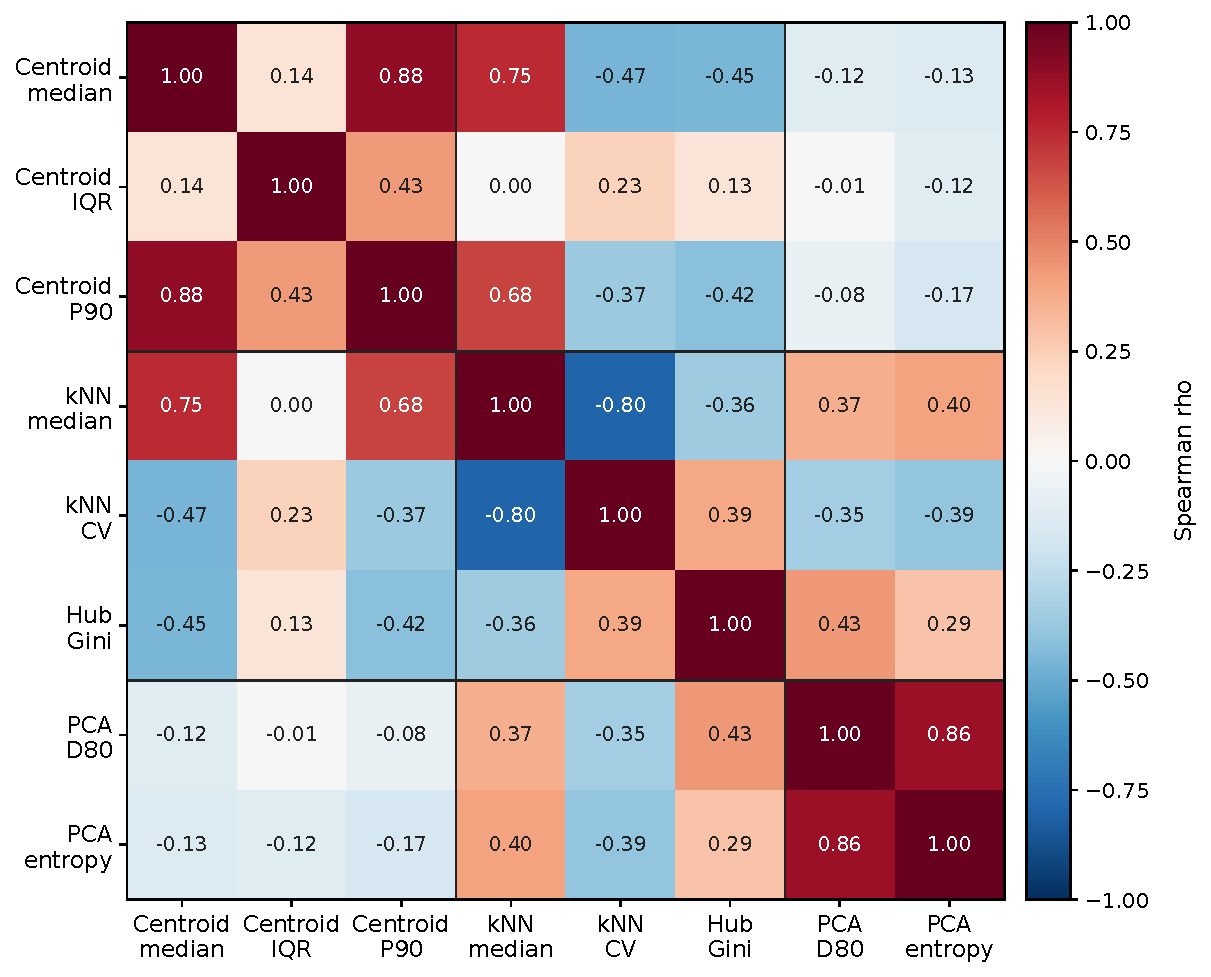
\includegraphics[width=0.78\textwidth]{figures/fig_06_structural_metric_spearman_correlation.pdf}
\end{figure}

\section{Domain Tendencies}

Static comparison uses one full-period structural morphology profile for each subfield. These profiles use the eight metrics defined in Chapter 3. Subfields are the direct measurement units; field and domain profiles are averages of standardized subfield profiles. In the heatmaps and boxplots, red indicates values above the median for that metric and blue indicates values below the median.

At the broadest scale, domains show tendencies. Physical Sciences are generally more dispersed and more spectrally extended. Health Sciences show tighter local neighborhoods and stronger local concentration. Social Sciences and Life Sciences are closer to the center of most metrics, with specific departures rather than one clear profile.

One possible interpretation is that Physical Sciences contain several well-developed research directions that use different concepts, methods, and technical languages. This could produce a document cloud with several broad directions rather than one compact centre. In Health Sciences, research may be organized more often around recurring diseases, treatments, clinical procedures, or highly connected reference topics. This could explain why papers form tighter local groups and why some papers occupy more central positions in the neighbourhood structure. The weaker domain-level patterns in Life Sciences and Social Sciences may reflect a mixture of very different fields whose profiles partly cancel out when they are averaged. These interpretations are plausible, but the metrics alone cannot identify the scientific causes behind the observed shapes.

\begin{figure}[H]
\centering
\caption[Domain-level morphological profiles]{Domain-level standardized structural morphology profiles. Values are visual contrasts across the four domain profiles, not inferential statistics.}
\label{fig:domain_metric_profile_heatmap}
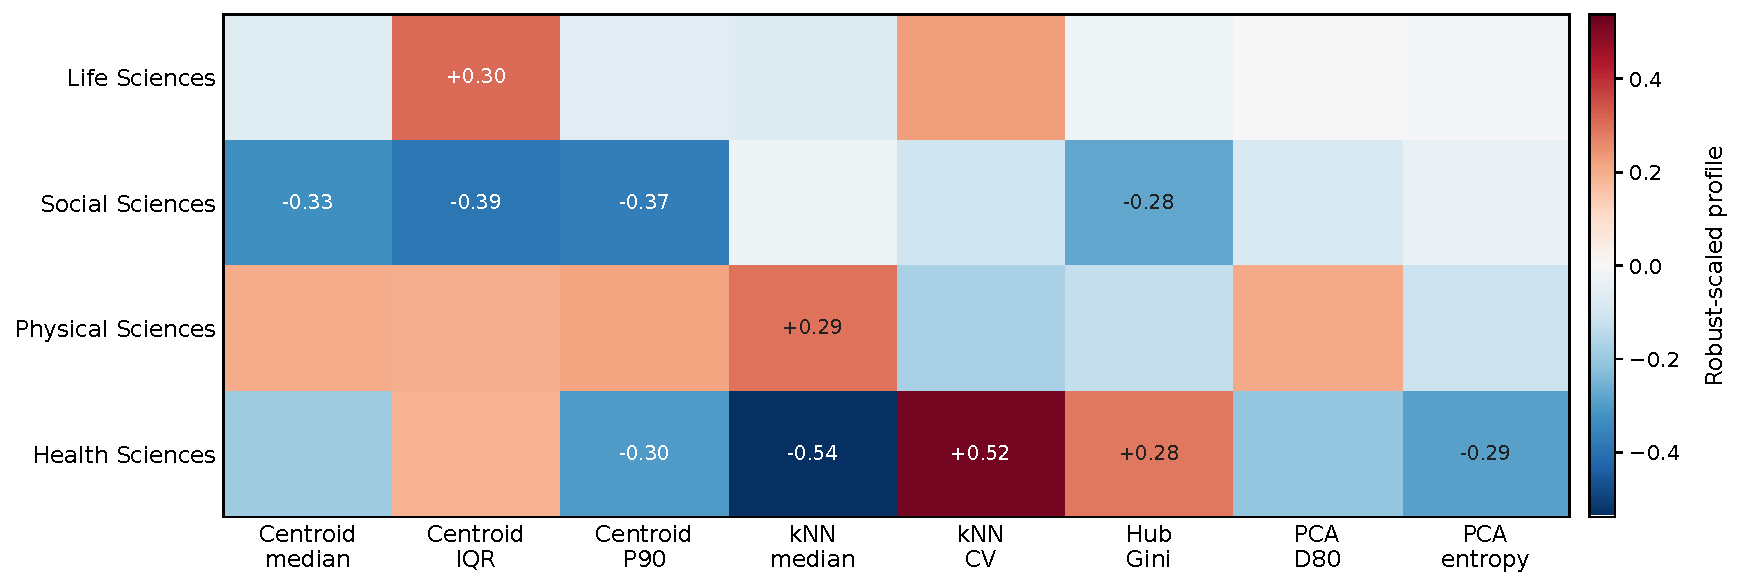
\includegraphics[width=\textwidth]{figures/fig_06_domain_metric_profile_heatmap.pdf}
\end{figure}

The domain view gives the first answer to the static part of the second research question: broad areas of science differ in shape. It is only a first answer. Four domain averages can hide strong variation among fields and subfields.

\section{Field and Subfield Heterogeneity}

Field profiles make the domain pattern less simple. Physical Sciences include dispersed fields such as Physics and Astronomy, Computer Science, Engineering, and Environmental Science. They also include more compact fields such as Energy and Mathematics. Health Sciences include dense fields such as Dentistry and Nursing, while Medicine sits closer to the center of the field distribution. Domains therefore show tendencies, not uniform morphologies.

The field-level profiles also show that fields can be unusual in different ways. Computer Science and Physics and Astronomy stand out mainly because their papers are spread more widely around the field centre. Chemistry, Materials Science, Engineering, and Environmental Science show larger distances between neighbouring papers, suggesting looser or more separated local research regions. Dentistry and Nursing show the opposite local pattern: their papers form tighter neighbourhoods, which may reflect research organized around recurring clinical problems, procedures, or treatments. Energy and Mathematics are important counterexamples within Physical Sciences because their more compact profiles differ from the broad pattern of their parent domain. Medicine remains closer to the middle of the field distribution, so the average Health Sciences profile is more strongly influenced by fields such as Dentistry, Nursing, and Health Professions. Figure 4.4 therefore helps distinguish whether a domain tendency is widely shared, driven by a few fields, or produced by opposite field profiles that partly cancel out when averaged.

\begin{figure}[H]
\centering
\caption[Field-level morphological profiles]{Field-level standardized structural morphology profiles. Rows are fields ordered by parent OpenAlex domain.}
\label{fig:field_metric_profile_heatmap}
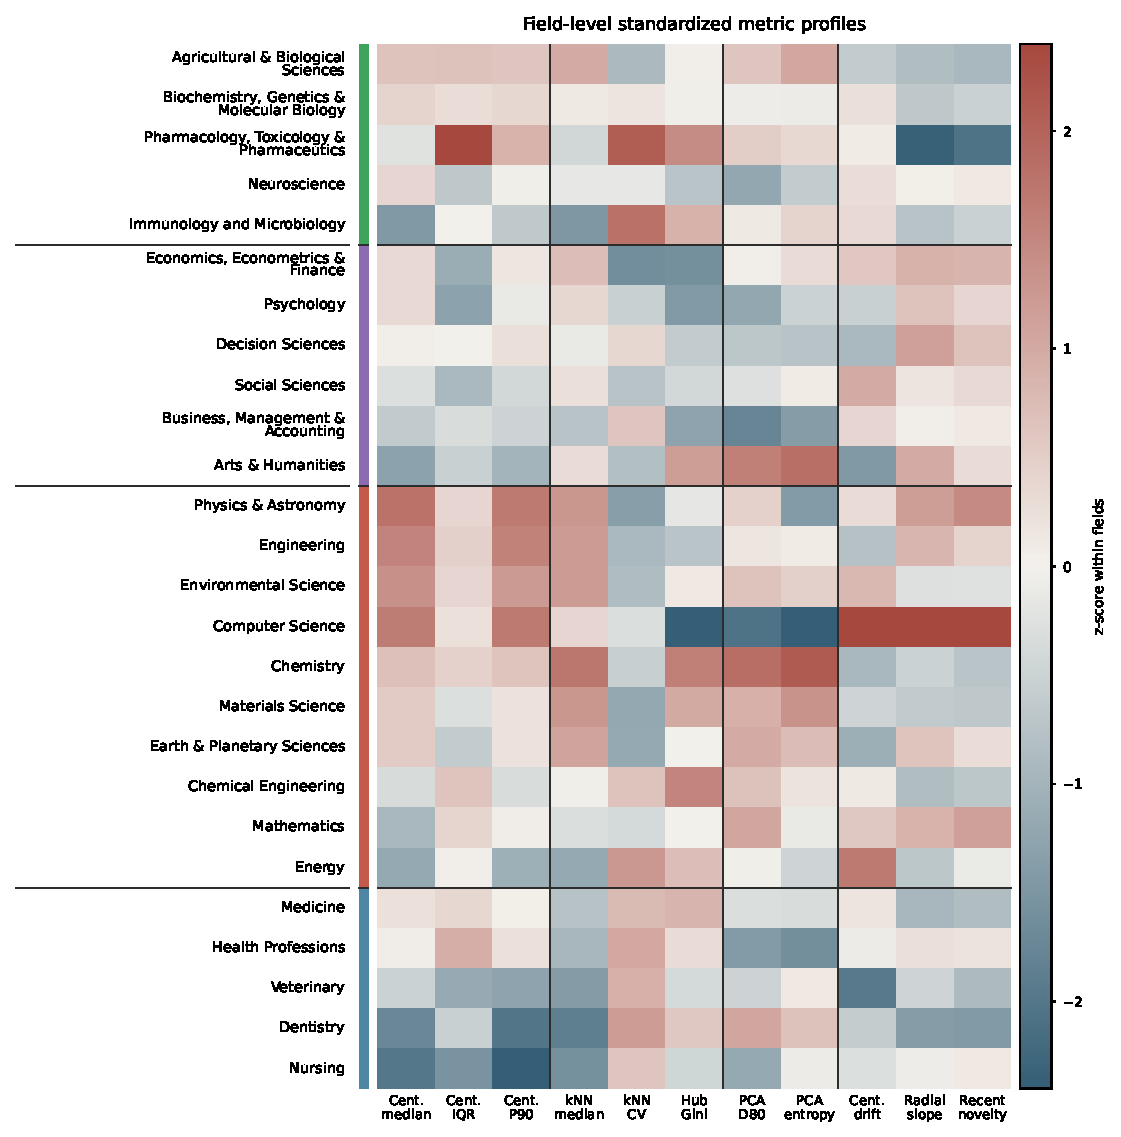
\includegraphics[width=\textwidth,height=0.78\textheight,keepaspectratio]{figures/fig_06_field_metric_profile_heatmap.pdf}
\end{figure}

The heatmap also reveals combinations that are hidden by a simple broad-versus-compact comparison. Computer Science has a wide overall spread, but low hubness and low spectral values, meaning that its variation is concentrated in fewer main directions and is not organized around a small set of dominant neighbouring papers. Arts and Humanities shows almost the opposite profile: it is relatively compact around its centre, but has higher hubness and spectral complexity. Pharmacology, Toxicology and Pharmaceutics stands out for a different reason, with very uneven distances both from the centre and within local neighbourhoods. These cases show that overall spread, local organization, hub concentration, and spectral structure can change independently. Two fields with a similar radius can therefore have very different internal structures.

\begin{figure}[H]
\centering
\caption[Subfield metric distributions by domain]{Subfield-level standardized metric distributions by domain for the eight structural metrics.}
\label{fig:subfield_metric_distributions_by_domain}
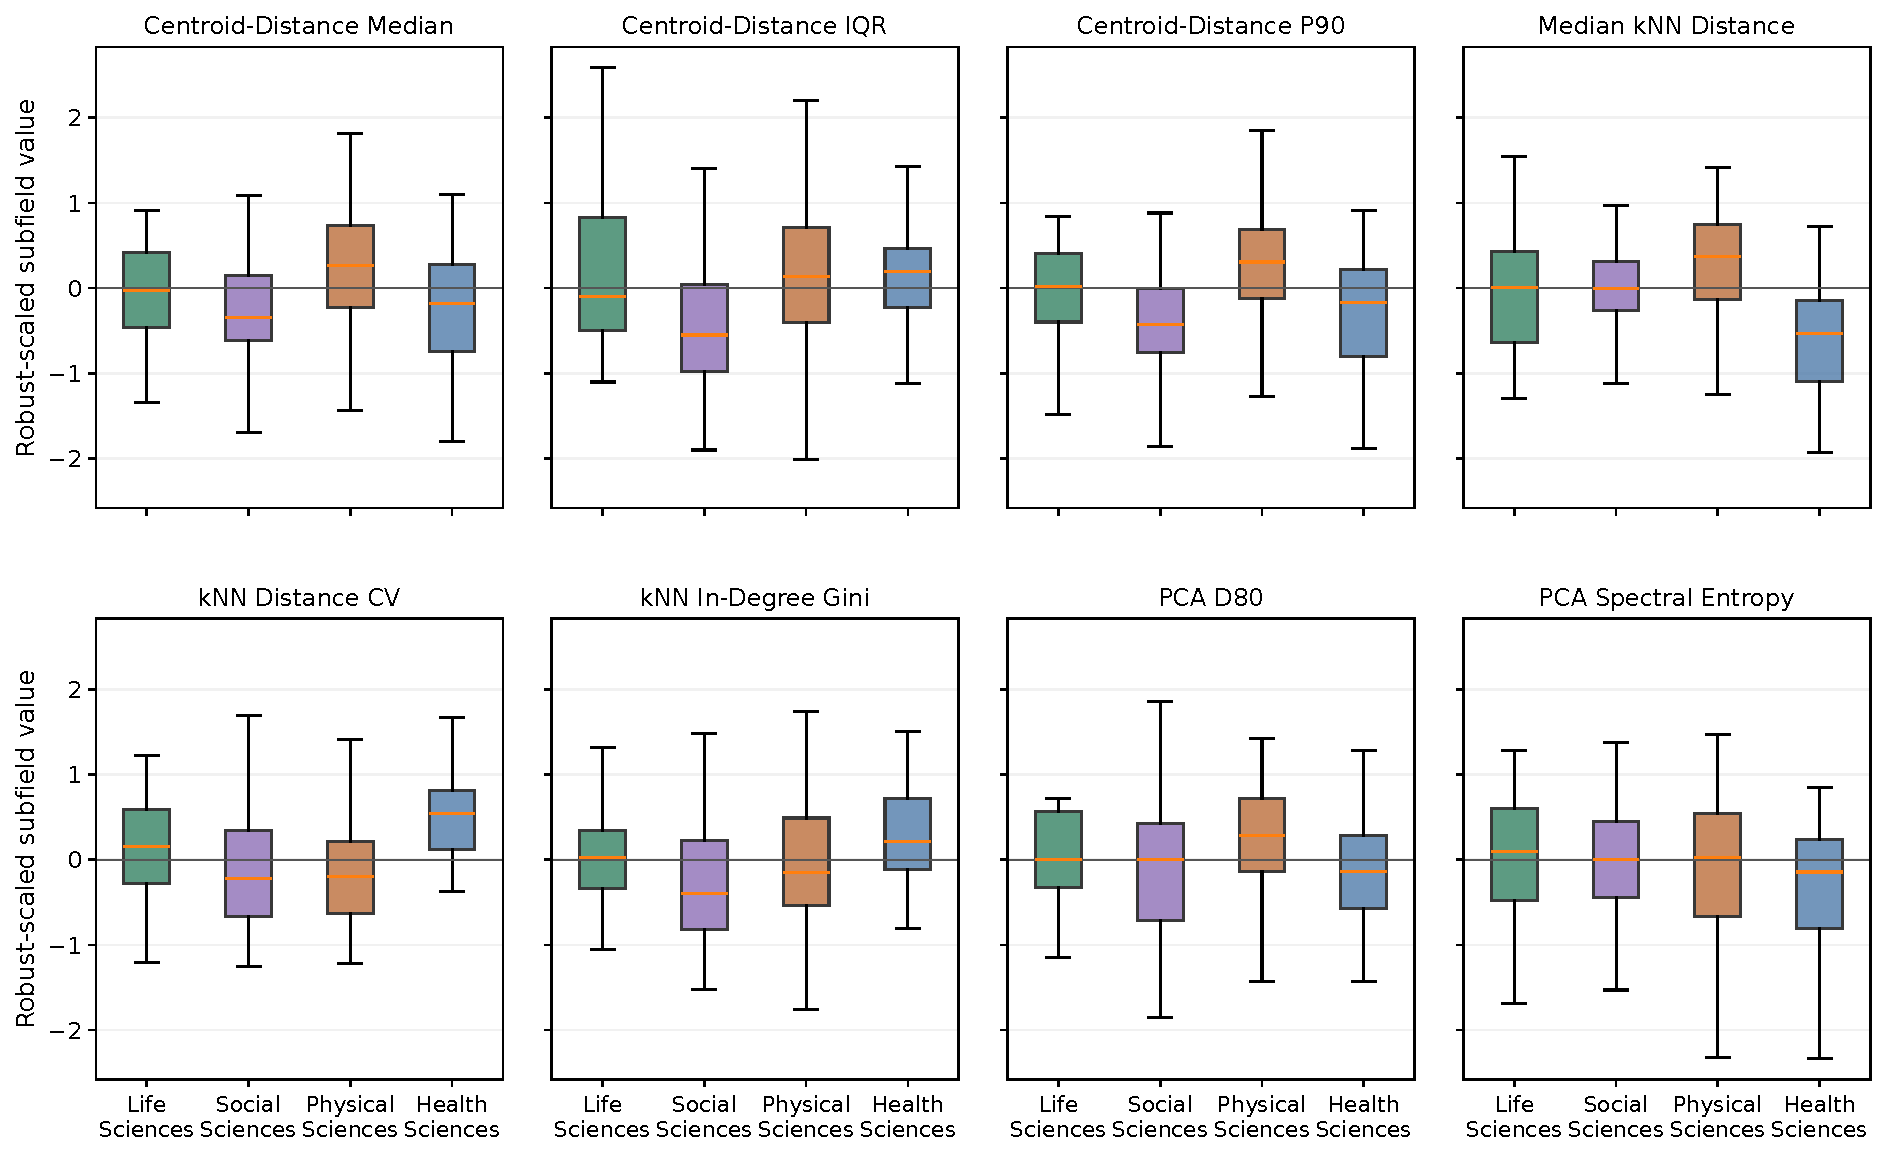
\includegraphics[width=\textwidth]{figures/fig_06_subfield_metric_distributions_by_domain.pdf}
\end{figure}

The boxplots show why morphology cannot be inferred from a domain label alone. Physical Sciences have the highest median subfield dispersion and kNN distance, but some physical subfields are compact. Health Sciences have lower local distances on average, but hubness varies widely. Social Sciences contain both compact applied areas and atypical humanities subfields. Field and subfield profiles are therefore not minor details after the domain result. They show where taxonomy and morphology partly separate.

\section{Metric Extremes and Profile Space}

Selected extremes make the same point with auditable cases. Nuclear and High Energy Physics and Artificial Intelligence sit at the high end of median centroid distance, while Applied Microbiology and Biotechnology and General Energy sit at the compact end. Molecular Medicine and Philosophy have unusually high centroid-distance IQR; Research and Theory and Algebra and Number Theory sit at the opposite end. Other metric families cut across these dispersion patterns. A field can be broad without being hub-dominated, and a compact field can still be locally uneven.

The standardized values in Table 4.1 show how unusual each subfield is relative to the rest of the sample. A value close to zero means that the subfield is near the median for that metric. Positive values indicate higher values and negative values indicate lower values. Because the scale is based on the median and the interquartile range, a score of +2 means two interquartile ranges above the median; it does not mean that the raw metric is twice as large. This also explains why some metrics can produce very large standardized scores even when their raw numerical range is small.

\begin{table}[H]
\centering
\caption{Selected subfield extremes in the static metric profiles}
\label{tab:extreme_subfields}
\scriptsize
\begingroup
\setlength{\tabcolsep}{2pt}
\begin{tabular}{@{}>{\raggedright\arraybackslash}p{0.17\textwidth} >{\raggedright\arraybackslash}p{0.25\textwidth} >{\raggedright\arraybackslash}p{0.25\textwidth} >{\raggedright\arraybackslash}p{0.21\textwidth}@{}}
\hline
\textbf{Metric} & \textbf{High end} & \textbf{Low end} & \textbf{Interpretation} \\
\hline
Median Centroid Distance & Nuclear and High Energy Physics; Artificial Intelligence; Electrical and Electronic Engineering & Applied Microbiology and Biotechnology; General Energy; Research and Theory & Broadest versus most compact semantic territories. \\
Median kNN Distance & Molecular Biology; Materials Chemistry; Biomedical Engineering & Applied Microbiology and Biotechnology; Internal Medicine; General Energy & Sparsest versus tightest local neighborhoods. \\
kNN In-Degree Gini & General Materials Science; Electrochemistry; Internal Medicine & Artificial Intelligence; Computer Vision and Pattern Recognition; Cognitive Neuroscience & Most versus least hub-concentrated neighborhood structure. \\
PCA D80 & Classics; Religious studies; Electrochemistry & Business and International Management; Computational Mathematics; Human Factors and Ergonomics & Most versus least distributed PCA variance. \\
Recent Novelty Score & Computer Vision and Pattern Recognition; Signal Processing; Human Factors and Ergonomics & Pharmaceutical Science; Molecular Medicine; Animal Science and Zoology & Recent work farthest from versus closest to the early semantic core. \\
\hline
\end{tabular}
\endgroup
\par\vspace{0.15cm}
\footnotesize\textit{Note.} Extremes are computed on raw metric values among the 241 eligible subfields; table entries list the top three subfields at each end of the selected metric.
\end{table}


These cases are not simply the largest or most productive subfields. Because the corpus is balanced, they appear in the table because the arrangement of their papers is unusual for a specific metric. The differences therefore reflect structure in the embedding space rather than publication volume.

The extremes also show why a single composite score would lose information. Human Factors and Ergonomics is unusual in spectral entropy, Applied Microbiology and Biotechnology in local-density variability, Classics and Religious studies in spectral extension, and Artificial Intelligence in low hub concentration. These are different kinds of structure. Keeping the metric families separate preserves those differences.

The exploratory PCA map in Figure~\ref{fig:metric_profile_pca_map} summarizes standardized structural profiles, not paper-level semantic locations. The first two axes explain 35.9 percent and 31.8 percent of the standardized profile variance. Domains overlap near the center. The most informative cases are specific subfields at the edges of the profile space.

\begin{figure}[H]
\centering
\caption[Subfield profile PCA map]{Exploratory PCA map of subfield structural morphology profiles. Points are subfields represented by the eight standardized structural metrics.}
\label{fig:metric_profile_pca_map}
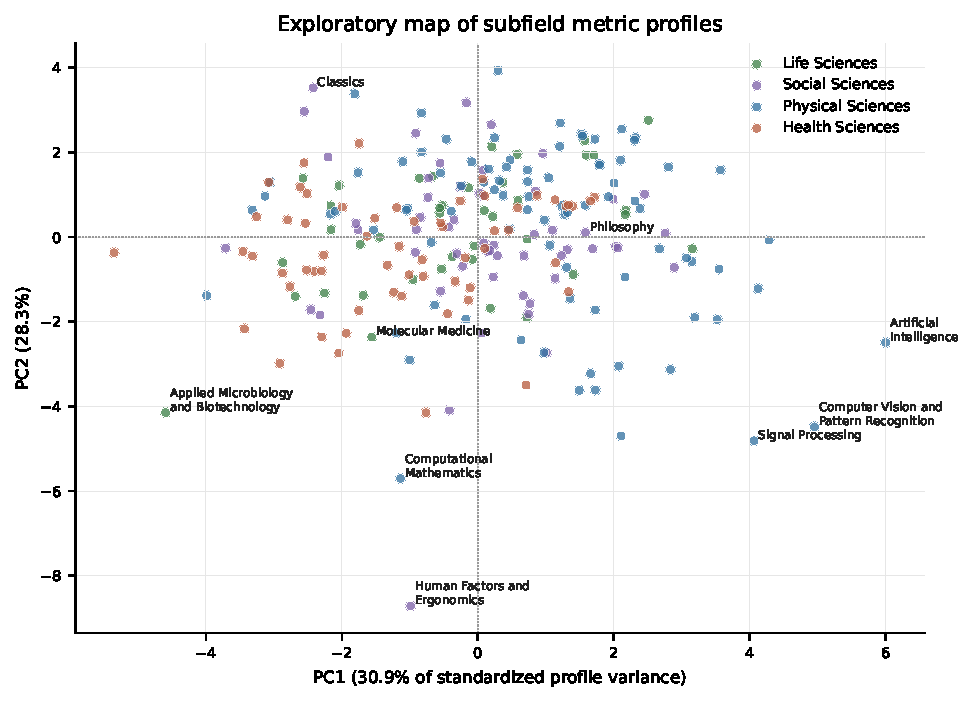
\includegraphics[width=\textwidth]{figures/fig_06_metric_profile_pca_map.pdf}
\end{figure}

The static result is clear but limited. Domains help orient the comparison, but they do not determine field shape. Broad domain tendencies coexist with large within-domain variation and cross-domain overlap in metric-profile space. Appendix~\ref{app:umap-atlas} keeps selected UMAP maps only as visual diagnostics. The next chapter therefore moves from full-period shape to structural change over time.
